\chapter{Analysis}

\subsection{Direction and consistency across environments}

Two patterns stand out. First, Open-Mindedness rises significantly in every single party environment ($\Delta$ between 0.65 and 0.83, all $p_t<0.05$), making it the only domain with a uniformly significant effect across the full political spectrum represented in the simulation. Second, every environment moves every domain in the same direction: all five parties increase Extraversion, Agreeableness, Conscientiousness, and Open-Mindedness relative to base, and all five decrease Neg.\ Emotionality. No party reverses the sign of any domain. This uniformity suggests that part of the measured effect may be attributable to a general simulation exposure effect, meaning agents becoming more socially confident and less anxious simply from having lived through a structured school day and interacted with peers, independent of which party's policies governed that day rather than a purely party-specific ideological effect. We return to this as a limitation in Chapter~\ref{limitations}.

Where the parties differ is in magnitude and in which domains cross the significance threshold (Appendix~\ref{appendix:paired_stats}):

\begin{itemize}
\item \textbf{Linke} produces the largest Agreeableness increase of any party ($\Delta=0.56$, $d=3.56$) and the largest decrease in Neg.\ Emotionality ($\Delta=-0.31$, $d=-2.98$), both significant. This is consistent with Die Linke's programme of non-selective schooling, individualised feedback instead of grades, and reduced homework (Section~1), which removes several common sources of peer competition and performance pressure.
\item \textbf{Gr\"une} is the only other party with a significant Neg.\ Emotionality decrease ($\Delta=-0.25$, $d=-3.66$) alongside a significant Agreeableness gain, matching its stated emphasis on inclusion and modern, participatory pedagogy.
\item \textbf{SPD} shows the strongest Open-Mindedness effect of all five parties ($\Delta=0.83$) and is one of only two environments with a significant Extraversion increase ($\Delta=0.21$, $p_t=0.030$), broadly consistent with its focus on educational mobility and opportunity.
\item \textbf{AfD} produces significant increases in Extraversion ($\Delta=0.44$, the largest of any party), Agreeableness, and Open-Mindedness. This is a counter-intuitive result given the party's traditional, discipline-oriented programme, and is discussed further in Chapter~\ref{limitations}.
\item \textbf{CDU} is the environment with the fewest significant shifts, only Open-Mindedness reaches significance. Point estimates for Conscientiousness (0.35) and Extraversion (0.38) are comparable in size to the other parties, but higher within-agent variance (larger $sd_{\Delta}$) keeps them below the significance threshold. This relative "flatness" is at least directionally consistent with a programme built around stability, performance standards, and the traditional multi-track structure.
\end{itemize}

Conscientiousness is the one domain that never reaches significance in any environment, despite positive point estimates throughout (0.31--0.40). Given paired Cohen's $d$ values in the 0.6--1.0 range, this looks like a power problem rather than a null effect: the true shift is plausibly non-zero, but $n=4$ students is not enough to detect a medium effect size reliably.

\section{Individual-Level Variation}
\label{sec:individual-level}

Group means can mask substantial disagreement between agents. Figure~\ref{fig:individual-heatmap} breaks the domain shifts down by agent (including the teacher, Katharina Weber) and environment.

\begin{figure}[htbp]
\centering
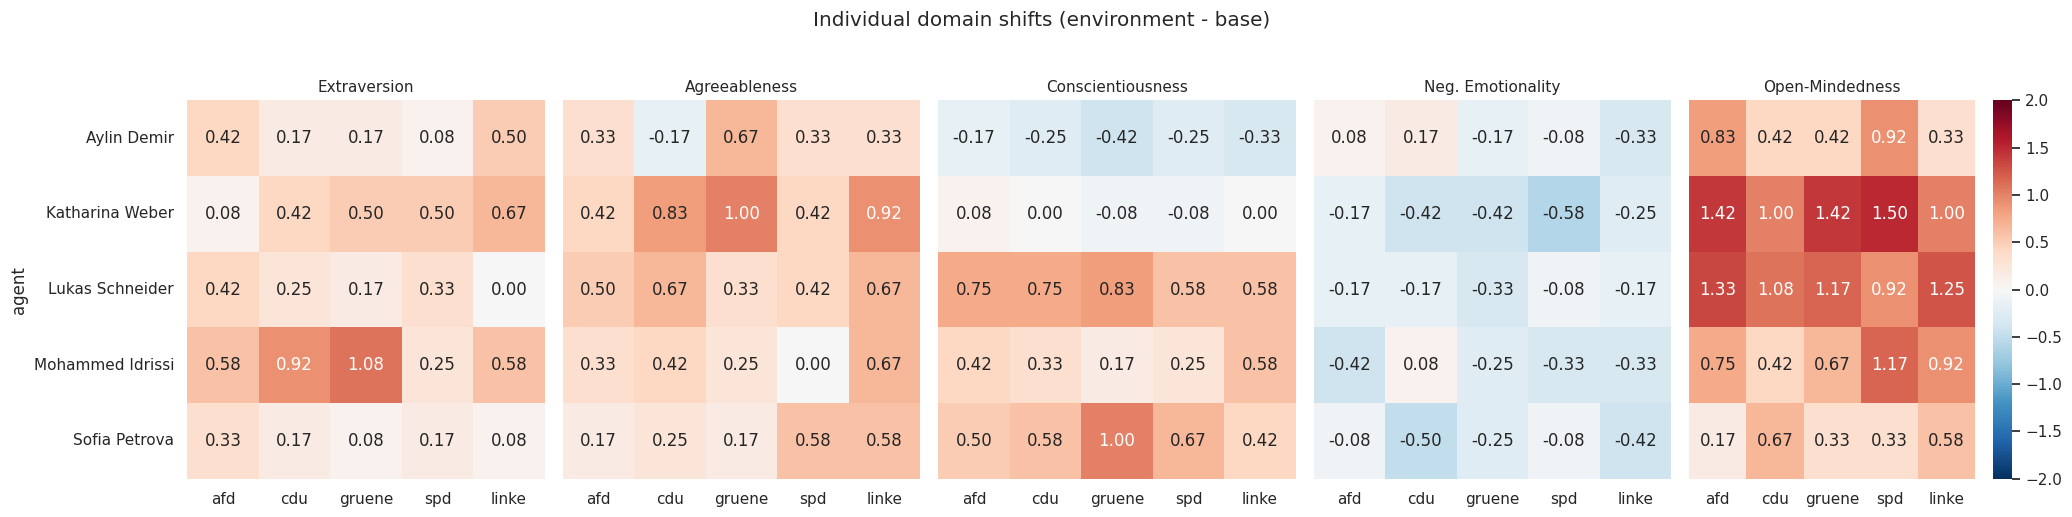
\includegraphics[width=\textwidth]{figures/individual_shift_heatmap.png}
\caption{Individual domain shifts (environment $-$ base) by agent. Katharina Weber is the teacher agent; the remaining four rows are the students used in Table~\ref{tab:paired-stats}.}
\label{fig:individual-heatmap}
\end{figure}

\begin{figure}[htbp]
\centering
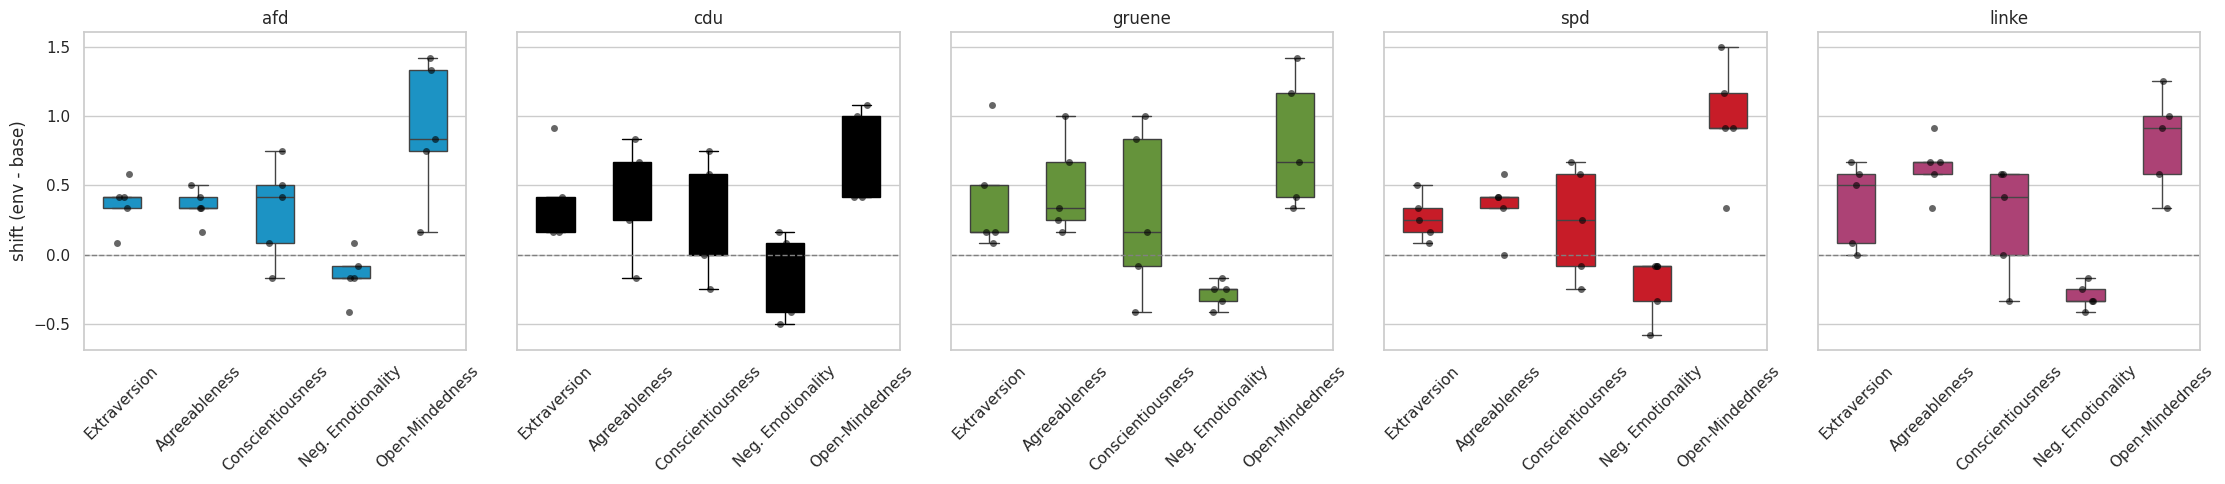
\includegraphics[width=\textwidth]{figures/spread_boxplot.png}
\caption{Spread of individual student shifts per domain, one panel per environment.}
\label{fig:spread}
\end{figure}

Three observations follow from the individual-level view. First, the teacher
agent, Katharina Weber, consistently shows the \emph{largest} Open-Mindedness
shift of any agent in every environment (1.00--1.50), well above the student
range (0.33--1.33). Since her role and daily schedule were rewritten for
each party to reflect that party's pedagogical philosophy, this is expected:
she is the agent most directly exposed to the ideological content of each
environment, and it registers most strongly on her open-mindedness score.

Second, the boxplots in Figure~\ref{fig:spread} show that
\textbf{Conscientiousness has the widest interquartile spread of any domain
in most environments} (e.g.\ CDU ranges from about $-0.5$ to $+0.75$), which
explains why it never reaches significance in Table~\ref{tab:paired-stats}
despite consistently positive medians: individual agents respond quite
differently to the same environment. Neg.\ Emotionality and Open-Mindedness,
by contrast, show comparatively tight, one-sided distributions (nearly all
individual shifts negative for Neg.\ Emotionality and positive for
Open-Mindedness), which is why those two domains yield the clearest
significant effects.

Third, no single student is a uniform outlier: each of the four students
(Sofia Petrova, Mohammed Idrissi, Lukas Schneider, Aylin Demir) shows at
least one domain/environment combination with a shift near zero or slightly
negative, even in domains where the group mean is strongly positive, e.g.\
Aylin Demir's Conscientiousness shift is negative in four of the five
environments while the group mean is positive throughout. This indicates
that the group-level effects in Section~4.1 are driven by a majority
tendency rather than by unanimous agreement among agents.

\section{Facet-Level Detail}

Figure~\ref{fig:facet-radar} disaggregates the five domains into their 15
constituent BFI-2 facets, plotting the group-mean facet profile for each
environment against the base measurement.

\begin{figure}[htbp]
\centering
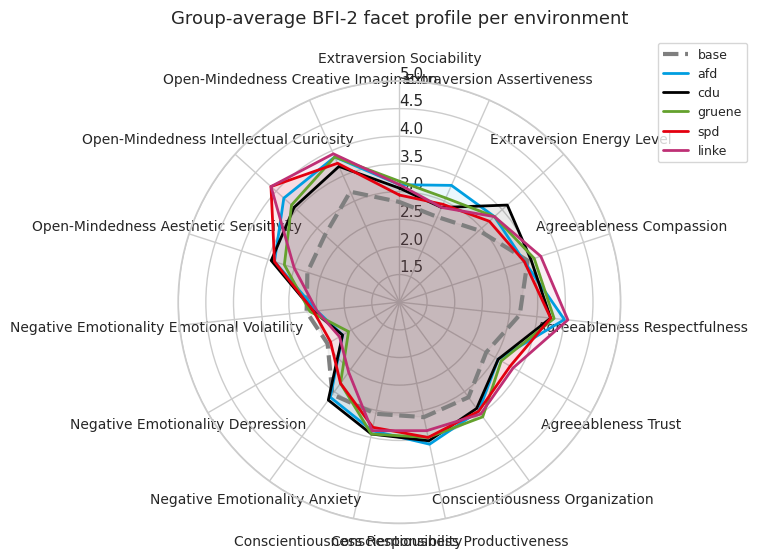
\includegraphics[width=0.75\textwidth]{figures/facet_radar.png}
\caption{Group-average BFI-2 facet profile per environment (15 facets, base vs.\ five party environments).}
\label{fig:facet-radar}
\end{figure}

The facet view shows that the domain-level Open-Mindedness effect is carried
primarily by \emph{Intellectual Curiosity} and \emph{Aesthetic Sensitivity},
which separate most clearly from the base profile across all five
environments, while \emph{Creative Imagination} shows a smaller gap. Within
Agreeableness, \emph{Respectfulness} shows the largest and most consistent
separation from base of the three facets — plausibly reflecting that a full
day inside any of the five structured party environments, each with its own
explicit classroom rules, increases agents' expressed respect for
those rules and for the teacher — while \emph{Trust} moves by comparatively
less. Within Conscientiousness, \emph{Organization} separates from base more
than \emph{Productiveness} or \emph{Responsibility}, consistent with the
domain-level result being real but individually noisy (Section~4.2). The
Negative Emotionality facets move together as a block, with \emph{Depression}
showing the clearest environment-vs-base gap and \emph{Anxiety} the
smallest, matching the domain-level finding that the overall Neg.\
Emotionality decrease is modest but directionally consistent.